\documentclass[11pt]{article}

% Language setting
\usepackage[turkish]{babel}
\usepackage{pythonhighlight}

\usepackage[a4paper,top=2cm,bottom=2cm,left=2cm,right=2cm,marginparwidth=2cm]{geometry}

% Useful packages
\usepackage{amsmath}
\usepackage{graphicx}
\usepackage[colorlinks=true, allcolors=blue]{hyperref}
\usepackage{verbatim}
\usepackage{fancyhdr} % for header and footer
\usepackage{titlesec}
\usepackage{parskip}

\setlength{\parindent}{0pt}

\titleformat{\subsection}[runin]{\bfseries}{\thesubsection}{1em}{}

\pagestyle{fancy} % activate the custom header/footer

% define the header/footer contents
\lhead{\small{23BLM-4014 Yapay Sinir Ağları Ara Sınav Soru ve Cevap Kağıdı}}
\rhead{\small{Dr. Ulya Bayram}}
\lfoot{}
\rfoot{}

% remove header/footer on first page
\fancypagestyle{firstpage}{
  \lhead{}
  \rhead{}
  \lfoot{}
  \rfoot{\thepage}
}
 

\title{Çanakkale Onsekiz Mart Üniversitesi, Mühendislik Fakültesi, Bilgisayar Mühendisliği Akademik Dönem 2022-2023\\
Ders: BLM-4014 Yapay Sinir Ağları/Bahar Dönemi\\ 
ARA SINAV SORU VE CEVAP KAĞIDI\\
Dersi Veren Öğretim Elemanı: Dr. Öğretim Üyesi Ulya Bayram}
\author{%
\begin{minipage}{\textwidth}
\raggedright
Öğrenci Adı Soyadı: Emre Gedük\\ % Adınızı soyadınızı ve öğrenci numaranızı noktaların yerine yazın
Öğrenci No: 190401070
\end{minipage}%
}

\date{14 Nisan 2023}

\begin{document}
\maketitle

\vspace{-.5in}
\section*{Açıklamalar:}
\begin{itemize}
    \item Vizeyi çözüp, üzerinde aynı sorular, sizin cevaplar ve sonuçlar olan versiyonunu bu formatta PDF olarak, Teams üzerinden açtığım assignment kısmına yüklemeniz gerekiyor. Bu bahsi geçen PDF'i oluşturmak için LaTeX kullandıysanız, tex dosyasının da yer aldığı Github linkini de ödevin en başına (aşağı url olarak) eklerseniz bonus 5 Puan! (Tavsiye: Overleaf)
    \item Çözümlerde ya da çözümlerin kontrolünü yapmada internetten faydalanmak, ChatGPT gibi servisleri kullanmak serbest. Fakat, herkesin çözümü kendi emeğinden oluşmak zorunda. Çözümlerinizi, cevaplarınızı aşağıda belirttiğim tarih ve saate kadar kimseyle paylaşmayınız. 
    \item Kopyayı önlemek için Github repository'lerinizin hiçbirini \textbf{14 Nisan 2023, saat 15:00'a kadar halka açık (public) yapmayınız!} (Assignment son yükleme saati 13:00 ama internet bağlantısı sorunları olabilir diye en fazla ekstra 2 saat daha vaktiniz var. \textbf{Fakat 13:00 - 15:00 arası yüklemelerden -5 puan!}
    \item Ek puan almak için sağlayacağınız tüm Github repository'lerini \textbf{en geç 15 Nisan 2023 15:00'da halka açık (public) yapmış olun linklerden puan alabilmek için!}
    \item \textbf{14 Nisan 2023, saat 15:00'dan sonra gönderilen vizeler değerlendirilmeye alınmayacak, vize notu olarak 0 (sıfır) verilecektir!} Son anda internet bağlantısı gibi sebeplerden sıfır almayı önlemek için assignment kısmından ara ara çözümlerinizi yükleyebilirsiniz yedekleme için. Verilen son tarih/saatte (14 Nisan 2023, saat 15:00) sistemdeki en son yüklü PDF geçerli olacak.
    \item Çözümlerin ve kodların size ait ve özgün olup olmadığını kontrol eden bir algoritma kullanılacaktır. Kopya çektiği belirlenen vizeler otomatikman 0 (sıfır) alacaktır. Bu nedenle çözümlerinizi ve kodlarınızı yukarıda sağladığım gün ve saatlere kadar kimseyle paylaşmayınız.
    \item Bu vizeden alınabilecek en yüksek not 100'dür. Toplam aldığınız puan 100'ü geçerse, aldığınız not 100'e sabitlenecektir.
    \item LaTeX kullanarak PDF oluşturanlar öz geçmişlerine LaTeX bildiklerini de eklemeyi unutmasınlar :)
    \item Bu vizedeki soruların çözümleri ve tex dosyası için istediğiniz kadar sayıda Github repository'si oluşturabilirsiniz. Sadece yukarıda belirttiğim tarihlerde (14 Nisan 2023 saat 15:00 ile 15 Nisan 2023 saat 15:00 arasında) public yapmayı/halka açmayı ve Github profilinizi de öz geçmişinize eklemeyi unutmayın :)
    \item Bilgisayarınıza hiçbir program kurmadan, Overleaf, Google Colab, Kaggle gibi ortamlar üzerinden bu vizeyi tamamlamanız mümkün. İyi çalışmalar!!
\end{itemize}

(Ekstra 5 puan) \url{OdevinTexDosyasınınGithubLinkiniburayakoyun.com}

\newpage
\section{(Toplam 10 Puan) Hopfield Networks:}

\subsection{(2 Puan)} \textbf{ChatGPT’ye size Hopfield Network’ler ile ilgili detaylı bilgi vermesini isteyin. Sorduğunuz soruyu, ChatGPT'nin çıkartığı cevabı aşağı koyun. Bu cevapta anlamadığınız terimleri de ChatGPT’ye sorup, sorduğunuz soruları ve ChatGPT’nin verdiği cevapları da sırayla aşağı koyun.}

\textbf{Hopfield networks nedir ayrıntılı bir şekilde bilgi verir misin ?} }

Hopfield ağları, sinir ağları olarak adlandırılan yapay sinir ağlarının bir türüdür. Bu ağlar, bellek ve optimizasyon problemlerinin çözümünde kullanılırlar. Bu tür ağlar, John Hopfield tarafından 1982 yılında önerilmiştir.

Hopfield ağları, geri beslemeli ağlar olarak adlandırılan bir sinir ağı tipidir. Geri besleme, bir ağın çıkışının, ağın girişindeki verileri değiştirebileceği anlamına gelir. Hopfield ağları, özellikle bellek yansıtmak için kullanılır. Bu nedenle, bir Hopfield ağı bir bellek gibi davranabilir ve öğrendiği örnekleri hatırlayabilir.

Hopfield ağları, nöronlar adı verilen işlem birimlerinden ve bunların birbirleriyle bağlantılarından oluşur. Bu bağlantılar, her bir nöronun diğer nöronlarla bağlantılı olduğu tam bağlantılı bir ağ oluşturur. Ayrıca, her nöron, diğer tüm nöronlarla bağlantılıdır.

Hopfield ağları, enerji fonksiyonları kullanarak çalışırlar. Enerji fonksiyonları, bir sistemin enerjisini hesaplamak için kullanılır. Hopfield ağlarında, enerji fonksiyonu, ağın belirli bir durumunun ne kadar iyi olduğunu belirler. Bu fonksiyon, ağın öğrenmesi ve hatırlaması için kullanılır.

Hopfield ağları, öğrenme ve hatırlama aşamalarından oluşur. Öğrenme aşamasında, ağa bellek örnekleri verilir ve ağ, bu örnekleri bellek olarak kaydeder. Hatırlama aşamasında, ağa bir girdi verilir ve ağ, bu girdiye en yakın bellek örneğini hatırlamaya çalışır.

Hopfield ağları, çözülemeyen birçok optimizasyon probleminin çözümünde kullanılabilir. Örneğin, seyahat satıcısı problemi, Hopfield ağları kullanılarak çözülebilir.

Hopfield ağları, yapay sinir ağları alanında önemli bir yere sahiptir ve birçok uygulama alanında kullanılmaktadır.

\textbf{Burada bahsettiğin bellek yansıtmak nedir ?}

Bellek yansıtmak, bir Hopfield ağının öğrenilen örnekleri hatırlayabilme yeteneğine sahip olması anlamına gelir. Hopfield ağları, bir örnek kümesi verildiğinde, bu örnekleri öğrenerek bir bellek haline getirebilirler. Daha sonra, ağa yeni bir girdi verildiğinde, ağ, öğrenilen örneklerden en yakın olanını hatırlamaya çalışır. Bu, bellek yansıtma olarak adlandırılır.

Örneğin, bir Hopfield ağına bir dizi resim verilebilir ve ağ, bu resimleri bellek olarak kaydedebilir. Daha sonra, ağa yeni bir resim verildiğinde, ağ, öğrenilen resimlerden en yakın olanını hatırlamaya çalışır. Bu, bellek yansıtma yeteneği sayesinde mümkün olur.

Bellek yansıtma yeteneği, birçok uygulama için yararlıdır. Örneğin, Hopfield ağları, tanıma sistemlerinde kullanılabilir. Bir Hopfield ağına bir dizi örnek verildiğinde, ağ, bu örneklerden en yakın olanını hatırlayabilir ve yeni bir girdi verildiğinde, ağ, bu girdinin hangi örnek ile en yakın olduğunu belirleyebilir. Bu, Hopfield ağlarının birçok uygulamada kullanılmasını mümkün kılar.

\textbf{Burada bahsettiğin enerji fonksiyonu tam olarak nedir ?}

Enerji fonksiyonu, Hopfield ağlarının çalışmasında önemli bir rol oynayan bir matematiksel fonksiyondur. Bu fonksiyon, ağın belirli bir durumunun enerjisini hesaplamak için kullanılır. Hopfield ağlarında, enerji fonksiyonu, ağın öğrenmesi ve hatırlaması için kullanılır.

Enerji fonksiyonu, ağın durumunu belirleyen nöron aktivasyonlarına ve bağlantı ağırlıklarına bağlıdır. Genellikle, enerji fonksiyonu, ağın belirli bir durumunda nöronlar arasındaki bağlantıların ne kadar uyumlu olduğunu ölçer. Uyumlu bağlantıların enerjisi daha düşükken, uyumsuz bağlantıların enerjisi daha yüksektir.

Enerji fonksiyonu, ağın öğrenmesi sırasında kullanılır. Öğrenme aşamasında, ağa bellek örnekleri verilir ve ağ, bu örnekleri bellek olarak kaydeder. Enerji fonksiyonu, ağın öğrenilen örnekleri hatırlamasına yardımcı olur ve öğrenme sırasında ağın enerjisi düşürülür.

Hatırlama aşamasında, ağa bir girdi verilir ve ağ, bu girdiye en yakın bellek örneğini hatırlamaya çalışır. Bu sırada, enerji fonksiyonu, ağın durumunun enerjisini hesaplar. Ağ, enerji fonksiyonunu minimize etmek için çaba gösterir ve hatırlanacak örneğe en yakın olan ağ durumunu bulmaya çalışır.

Bir örnek vermek gerekirse, Hopfield ağları, veri sıkıştırma ve desen tanıma gibi birçok uygulama alanında kullanılır. Örneğin, bir Hopfield ağına bir dizi resim verildiğinde, ağ bu resimleri bellek olarak kaydedebilir ve daha sonra bu resimlere benzer yeni bir resim verildiğinde, ağ, enerji fonksiyonunu minimize ederek, en yakın örneği hatırlayabilir. Bu sayede, veri sıkıştırma ve desen tanıma işlemleri yapılabilir.

\subsection{(8 Puan)} \textbf{ChatGPT’nin açıklamalarından ne anladığınızı buraya kendi kelimelerinizle özetleyin. Örneğin ``Hopfield Network nedir? Ne işe yarar? Neden bilmemiz gerekir bunu? Gerçek hayatta kullanılıyor mu?'' gibi. Anlamadığınız kısımlar varsa ve ChatGPT’nin açıklamaları yeterli gelmezse internet dahil farklı kaynaklardan araştırıp, bilgilerin doğruluğunu sorgulamakta serbestsiniz. Konuyu doğru anlayıp anlamamanız puana etki edecektir. Kullandığınız kaynakları da belirtin!}

Hopfield ağları bir tür yapay sinir ağıdır. Hopfield ağlarında tüm nöronlar birbirleri ile bağlantılıdır. Hopfield ağları verilen girdi örneklerini öğrenir ve bu örnekleri hatırlayabilir. Örneğin bir girdi verdik. Hopfield ağları daha önce öğrendiklerinden bu girdiye en yakın olanı hatırlar. Bu öğrenme ve hatırlama işlemi enerji fonksiyonu ile yapılır. Enerji fonksiyonu nöronlar arasındaki bağlantının ne kadar uyumlu olduğunu gösterir. Enerji fonksiyonunun düşük olması ağın belli bir durumunun uyumlu olduğunu gösterir. Yani verilen girdinin hatırlanacak şeye yakın olduğunu gösterir. Enerji yüksekse de hatırlanacak şeye ağın ağın daha uzak olduğunu belirtir. Hopfield ağları genelde optimizasyon problemleri çözümünde ve tanıma sistemlerinde kullanılır.

\textbf{Araştırma yaparken kullandığım diğer kaynaklar:}

https://towardsdatascience.com/hopfield-networks-neural-memory-machines-4c94be821073




\section{(Toplam 10 Puan) Boltzman Machine:}

\subsection{(2 Puan)} \textbf{ChatGPT’ye size Boltzman Machine ilgili detaylı bilgi vermesini isteyin. Sorduğunuz soruyu, ChatGPT'nin çıkartığı cevabı aşağı koyun. Bu cevapta anlamadığınız terimleri de ChatGPT’ye sorup, sorduğunuz soruları ve ChatGPT’nin verdiği cevapları da sırayla aşağı koyun.}

\textbf{Boltzman machine hakkında detaylı bilgi verir misin ?}

Boltzmann makineleri, makine öğrenmesinde kullanılan olasılıksal bir modelleme teknolojisidir. İsimlerini ünlü fizikçi Ludwig Boltzmann'dan almışlardır.

Boltzmann makineleri, genellikle sinir ağları olarak tanımlanan bir dizi birimden oluşur. Bu birimler, girdileri ve çıktıları olan nöronlara benzerler. Ancak, Boltzmann makineleri, her birimden birbirleriyle bağlantılar bulunan bir ağ oluşturur. Bu bağlantılar, birimin aktivasyon durumuna göre güçlü veya zayıf olabilir.

Boltzmann makineleri, bir veri kümesini analiz ederek, verinin olası yapısal özelliklerini keşfetmeye çalışırlar. Bunun için, birimlerin aktivasyon durumuna dayalı olarak bir olasılık dağılımı oluştururlar. Bu olasılık dağılımı, veri kümesinin özelliklerine göre ayarlanır.

Bir Boltzmann makinesi, iki tür birim içerir: gizli birimler ve görünür birimler. Gizli birimler, sadece diğer gizli birimlerle bağlantılıdır ve girdi olarak veri kümesinin bir özeti olarak kabul edilen görünür birimler tarafından etkilenir. Gizli birimlerin durumunu belirlemek için, her bir gizli birim, diğer gizli birimlerin aktivasyon durumlarına ve görünür birimlerin durumuna göre hesaplanan bir olasılık dağılımına göre aktivasyon durumunu belirler.

Bir Boltzmann makinesinin eğitimi, veri kümesinin olası özelliklerinin keşfedilmesiyle ilgilidir. Bu amaçla, makineye bir öğrenme veri kümesi sağlanır ve makine, veri kümesine uygun bir olasılık dağılımı oluşturmak için ağırlıkları ayarlar.

Boltzmann makineleri, özellikle ölçeklenebilir olmaları nedeniyle büyük ve karmaşık veri kümeleri üzerinde çalışmak için kullanışlıdır. Ayrıca, derin öğrenme algoritmalarının temelini oluştururlar ve özellikle resim, doğal dil işleme ve konuşma tanıma gibi alanlarda başarılı sonuçlar verirler.

\textbf{Burada bahsettiğin birimin aktivasyon durumu nedir ?}

Boltzmann makinelerindeki birimin aktivasyon durumu, o birimin ne kadar "aktif" olduğunu belirten bir değerdir. Aktivasyon durumu, genellikle 0 veya 1 gibi bir sayıyla ifade edilir ve birimin işlevselliğini belirler.

Birimin aktivasyon durumu, ağın diğer birimleriyle olan bağlantılarına bağlı olarak hesaplanır. Bu bağlantılar, ağın öğrenme işlemindeki temel unsurlardır ve birimlerin birbirleriyle etkileşim kurmalarına ve birbirlerini etkilemelerine izin verir.

Birimin aktivasyon durumu, Boltzmann makinelerinde olasılık dağılımlarının hesaplanmasında önemlidir. Birimin aktivasyon durumuna bağlı olarak, diğer birimlerin aktivasyon durumları ve girdi değerleri ile birlikte, birimin olası çıktısı belirlenir. Bu sayede, veri kümesinin yapısal özelliklerini belirlemek ve keşfetmek için gerekli olan olasılık dağılımı oluşturulur.

Birimin aktivasyon durumu ayrıca, ağın öğrenme sürecinde kullanılan geriye yayılım algoritması gibi tekniklerde de önemlidir. Bu algoritmalar, hata değerlerinin ağın her bir birimine geriye doğru yayılması yoluyla, ağın ağırlıklarının ve bağlantılarının ayarlanmasını sağlar. Bu süreçte, her bir birimin aktivasyon durumu ve hata değeri hesaplanarak, ağın öğrenme sürecindeki rolü belirlenir.

Sonuç olarak, Boltzmann makinelerindeki birimin aktivasyon durumu, ağın işleyişinde temel bir rol oynar ve veri kümesinin özelliklerini keşfetmek için kullanılır.

\subsection{(8 Puan)} \textbf{ChatGPT’nin açıklamalarından ne anladığınızı buraya kendi kelimelerinizle özetleyin. Örneğin ``Boltzman Machine nedir? Ne işe yarar? Neden bilmemiz gerekir bunu? Gerçek hayatta kullanılıyor mu?'' gibi. Anlamadığınız kısımlar varsa ve ChatGPT’nin açıklamaları yeterli gelmezse internet dahil farklı kaynaklardan araştırıp, bilgilerin doğruluğunu sorgulamakta serbestsiniz. Konuyu doğru anlayıp anlamamanız puana etki edecektir. Kullandığınız kaynakları da belirtin!}

Boltzman makineleri, bir yapar sinir ağı türüdür. Bir dizi nöronlardan oluşur.  Gizli ve gözlemlenebilir olmak üzere iki tür birime sahiptir. Bu birimler, veri kümesinin özelliklerini belirlemek için kullanılır. İlk olarak rastgele durum atanır ve ağırlıklar belirlenir. Daha sonra ağırlıklar sürekli olarak optimize edilir. Bu şekilde örneğin girdi olarak bir resim veririz ardından boltzman makineleri bu resmin özelliklerini öğrenir ve benzer resimler oluşturabilir. Boltzman makineleri genellikle resim, NLP ve konuşma tanıma gibi alanlarda kullanılır.

\section{(Toplam 10 Puan) Markov Assumption ve Markov Chain:}

\subsection{(2 Puan)} \textbf{ChatGPT’ye size Markov assumption ve Markov Chain ilgili detaylı bilgi vermesini isteyin. Sorduğunuz soruyu, ChatGPT'nin çıkartığı cevabı aşağı koyun. Bu cevapta anlamadığınız terimleri de ChatGPT’ye sorup, sorduğunuz soruları ve ChatGPT’nin verdiği cevapları da sırayla aşağı koyun.}

\textbf{markov assumption ve markov chain hakkında detaylı bilgi verir misin ?}


Markov varsayımı, gelecekteki bir olayın olasılığının, sadece o anki durumun (veya geçmiş durumların) belirli bir noktasını, yani son birkaç olayı etkilediğini ifade eder. Başka bir deyişle, bir olayın oluşma olasılığı, sadece son birkaç olaya bağlıdır ve daha önceki olaylar bu olasılığı etkilemez.

Markov zinciri, Markov varsayımı ile tanımlanan bir olasılık sürecidir. Markov zinciri, bir dizi olası durumdan oluşur ve her bir durumun, sonraki durumun oluşma olasılığı, sadece o anki durumdan bağımsızdır ve sadece son birkaç durumdan etkilenir.

Markov zinciri, özellikle zaman içinde değişen bir sistem veya olayların modellenmesi için kullanılır. Örneğin, hava durumu veya finansal piyasalar gibi sürekli değişen sistemler, Markov zincirleri ile modelleme yapılabilir. Markov zincirleri ayrıca, sıralı verilerin modellemesi, n-gram dil modelleri, robotların hareketlerinin modellemesi gibi birçok farklı alanda kullanılır.

Markov zinciri, bir başlangıç durumu ile başlar ve belirli bir dizi durum oluşturur. Bu durumların her biri, sonraki durumların oluşma olasılığını belirleyen bir geçiş matrisi ile ilişkilidir. Geçiş matrisi, bir durumun, diğer duruma geçme olasılığını belirtir. Markov zincirleri, sürekli veya ayrık durumlar için kullanılabilir ve ayrık durumlar, genellikle bir sayı dizisi veya sembollerle temsil edilir.

\textbf{Yukarıdaki cevapta belirttiğin geçiş durumu tam olarak nedir ?}

Markov zincirinde, bir durumdan diğer duruma geçişler, "geçiş durumları" olarak adlandırılır. Geçiş durumları, durumların belirli bir zamanda sahip olabilecekleri farklı değerler arasındaki değişiklikleri temsil eder.

Geçiş durumları, geçiş matrisinde belirtilen olasılıklara göre gerçekleşir. Bu matris, her bir durumun, sonraki durumlara geçiş olasılıklarını gösteren bir matristir.

\subsection{(8 Puan)} \textbf{ChatGPT’nin açıklamalarından ne anladığınızı buraya kendi kelimelerinizle özetleyin. Örneğin ``Markov assumption ve Markov Chain nedir? Ne işe yarar? Neden bilmemiz gerekir bunu? Gerçek hayatta kullanılıyor mu?'' gibi. Anlamadığınız kısımlar varsa ve ChatGPT’nin açıklamaları yeterli gelmezse internet dahil farklı kaynaklardan araştırıp, bilgilerin doğruluğunu sorgulamakta serbestsiniz. Konuyu doğru anlayıp anlamamanız puana etki edecektir. Kullandığınız kaynakları da belirtin!}

Markov assumption, gelecekte bir olayın gerçekleşme olasılığının son birkaç olaya bağlı olduğunu, geçmişteki olayların olasılığı etkilemediğini söylüyor. Markov zinciri de markov assumption mantığı ile oluşturulan bir dizi olası durumdur. Örneğin bugün yağmur yağıyor olsun. Hava durumu tahmininde bu bilgi yarın yağmur yağma olasılığını arttırabilir. Çünkü Markov zincirinde geçmiş verilerden bağımsız olarak bir sonraki durumun  değeri sadece mevcut durumdaki değere
bağlı olarak değişmektedir . Bu verdiğim örnekte mevcut durum bugünün yağmurlu olmasıdır ve bir sonraki durumun olasılığını geçmişteki diğer veriler etkilemez sadece mevcut durum etkiler.
Aynı zamanda Markov zinciri, robotların hareketlerinin modellenmesi, finans ve hava durumu sistemlerinde kullanılır.

\section{(Toplam 20 Puan) Feed Forward:}
 
\begin{itemize}
    \item Forward propagation için, input olarak şu X matrisini verin (tensöre çevirmeyi unutmayın):\\
    $X = \begin{bmatrix}
        1 & 2 & 3\\
        4 & 5 & 6
        \end{bmatrix}$
    Satırlar veriler (sample'lar), kolonlar öznitelikler (feature'lar).
    \item Bir adet hidden layer olsun ve içinde tanh aktivasyon fonksiyonu olsun
    \item Hidden layer'da 50 nöron olsun
    \item Bir adet output layer olsun, tek nöronu olsun ve içinde sigmoid aktivasyon fonksiyonu olsun
\end{itemize}

Tanh fonksiyonu:\\
$f(x) = \frac{exp(x) - exp(-x)}{exp(x) + exp(-x)}$
\vspace{.2in}

Sigmoid fonksiyonu:\\
$f(x) = \frac{1}{1 + exp(-x)}$

\vspace{.2in}
 \textbf{Pytorch kütüphanesi ile, ama kütüphanenin hazır aktivasyon fonksiyonlarını kullanmadan, formülünü verdiğim iki aktivasyon fonksiyonunun kodunu ikinci haftada yaptığımız gibi kendiniz yazarak bu yapay sinir ağını oluşturun ve aşağıdaki üç soruya cevap verin.}
 
\subsection{(10 Puan)} \textbf{Yukarıdaki yapay sinir ağını çalıştırmadan önce pytorch için Seed değerini 1 olarak set edin, kodu aşağıdaki kod bloğuna ve altına da sonucu yapıştırın:}

% Latex'de kod koyabilirsiniz python formatında. Aşağıdaki örnekleri silip içine kendi kodunuzu koyun
\begin{python}
import torch
torch.manual_seed(1)

x = torch.tensor([[1, 2, 3], [4, 5, 6]], dtype=torch.float)

inputSize = x.shape[1]
hiddenSize = 50
outputSize = 1

w1 = torch.randn(inputSize, hiddenSize, dtype=torch.float)
b1 = torch.randn(hiddenSize, dtype=torch.float)
w2 = torch.randn(hiddenSize, outputSize, dtype=torch.float)
b2 = torch.randn(outputSize, dtype=torch.float)

def tanh(x):
    return (torch.exp(x) - torch.exp(-x)) / (torch.exp(x) + torch.exp(-x))

def sigmoid(x):
    return 1 / (1 + torch.exp(-x))

hiddenInput = torch.matmul(x, w1) + b1
hiddenOutput = tanh(hiddenInput)
outputInput = torch.matmul(hiddenOutput, w2) + b2
output = sigmoid(outputInput)

print(output)
\end{python}

tensor([[0.0498],
        [0.0075]])

\subsection{(5 Puan)} \textbf{Yukarıdaki yapay sinir ağını çalıştırmadan önce Seed değerini öğrenci numaranız olarak değiştirip, kodu aşağıdaki kod bloğuna ve altına da sonucu yapıştırın:}

\begin{python}
import torch
torch.manual_seed(190401070)

x = torch.tensor([[1, 2, 3], [4, 5, 6]], dtype=torch.float)

inputSize = x.shape[1]
hiddenSize = 50
outputSize = 1

w1 = torch.randn(inputSize, hiddenSize, dtype=torch.float)
b1 = torch.randn(hiddenSize, dtype=torch.float)
w2 = torch.randn(hiddenSize, outputSize, dtype=torch.float)
b2 = torch.randn(outputSize, dtype=torch.float)

def tanh(x):
    return (torch.exp(x) - torch.exp(-x)) / (torch.exp(x) + torch.exp(-x))

def sigmoid(x):
    return 1 / (1 + torch.exp(-x))

hiddenInput = torch.matmul(x, w1) + b1
hiddenOutput = tanh(hiddenInput)
outputInput = torch.matmul(hiddenOutput, w2) + b2
output = sigmoid(outputInput)

print(output)
\end{python}

tensor([[0.0105],
        [0.0001]])

\subsection{(5 Puan)} \textbf{Kodlarınızın ve sonuçlarınızın olduğu jupyter notebook'un Github repository'sindeki linkini aşağıdaki url kısmının içine yapıştırın. İlk sayfada belirttiğim gün ve saate kadar halka açık (public) olmasın:}
% size ait Github olmak zorunda, bu vize için ayrı bir github repository'si açıp notebook'u onun içine koyun. Kendine ait olmayıp da arkadaşının notebook'unun linkini paylaşanlar 0 alacak.

\url{https://github.com/EMREEGEDUKK/feedForwardPytorch/blob/main/FeedForward.ipynb}

\section{(Toplam 40 Puan) Multilayer Perceptron (MLP):} 
\textbf{Bu bölümdeki sorularda benim vize ile beraber paylaştığım Prensesi İyileştir (Cure The Princess) Veri Seti parçaları kullanılacak. Hikaye şöyle (soruyu çözmek için hikaye kısmını okumak zorunda değilsiniz):} 

``Bir zamanlar, çok uzaklarda bir ülkede, ağır bir hastalığa yakalanmış bir prenses yaşarmış. Ülkenin kralı ve kraliçesi onu iyileştirmek için ellerinden gelen her şeyi yapmışlar, ancak denedikleri hiçbir çare işe yaramamış.

Yerel bir grup köylü, herhangi bir hastalığı iyileştirmek için gücü olduğu söylenen bir dizi sihirli malzemeden bahsederek kral ve kraliçeye yaklaşmış. Ancak, köylüler kral ile kraliçeyi, bu malzemelerin etkilerinin patlayıcı olabileceği ve son zamanlarda yaşanan kuraklıklar nedeniyle bu malzemelerden sadece birkaçının herhangi bir zamanda bulunabileceği konusunda uyarmışlar. Ayrıca, sadece deneyimli bir simyacı bu özelliklere sahip patlayıcı ve az bulunan malzemelerin belirli bir kombinasyonunun prensesi iyileştireceğini belirleyebilecekmiş.

Kral ve kraliçe kızlarını kurtarmak için umutsuzlar, bu yüzden ülkedeki en iyi simyacıyı bulmak için yola çıkmışlar. Dağları tepeleri aşmışlar ve nihayet "Yapay Sinir Ağları Uzmanı" olarak bilinen yeni bir sihirli sanatın ustası olarak ün yapmış bir simyacı bulmuşlar.

Simyacı önce köylülerin iddialarını ve her bir malzemenin alınan miktarlarını, ayrıca iyileşmeye yol açıp açmadığını incelemiş. Simyacı biliyormuş ki bu prensesi iyileştirmek için tek bir şansı varmış ve bunu doğru yapmak zorundaymış. (Original source: \url{https://www.kaggle.com/datasets/unmoved/cure-the-princess})

(Buradan itibaren ChatGPT ve Dr. Ulya Bayram'a ait hikayenin devamı)

Simyacı, büyülü bileşenlerin farklı kombinasyonlarını analiz etmek ve denemek için günler harcamış. Sonunda birkaç denemenin ardından prensesi iyileştirecek çeşitli karışım kombinasyonları bulmuş ve bunları bir veri setinde toplamış. Daha sonra bu veri setini eğitim, validasyon ve test setleri olarak üç parçaya ayırmış ve bunun üzerinde bir yapay sinir ağı eğiterek kendi yöntemi ile prensesi iyileştirme ihtimalini hesaplamış ve ikna olunca kral ve kraliçeye haber vermiş. Heyecanlı ve umutlu olan kral ve kraliçe, simyacının prensese hazırladığı ilacı vermesine izin vermiş ve ilaç işe yaramış ve prenses hastalığından kurtulmuş.

Kral ve kraliçe, kızlarının hayatını kurtardığı için simyacıya krallıkta kalması ve çalışmalarına devam etmesi için büyük bir araştırma bütçesi ve çok sayıda GPU'su olan bir server vermiş. İyileşen prenses de kendisini iyileştiren yöntemleri öğrenmeye merak salıp, krallıktaki üniversitenin bilgisayar mühendisliği bölümüne girmiş ve mezun olur olmaz da simyacının yanında, onun araştırma grubunda çalışmaya başlamış. Uzun yıllar birlikte krallıktaki insanlara, hayvanlara ve doğaya faydalı olacak yazılımlar geliştirmişler, ve simyacı emekli olduğunda prenses hem araştırma grubunun hem de krallığın lideri olarak hayatına devam etmiş.

Prenses, kendisini iyileştiren veri setini de, gelecekte onların izinden gidecek bilgisayar mühendisi prensler ve prensesler başkalarına faydalı olabilecek yapay sinir ağları oluşturmayı öğrensinler diye halka açmış ve sınavlarda kullanılmasını salık vermiş.''

\textbf{İki hidden layer'lı bir Multilayer Perceptron (MLP) oluşturun beşinci ve altıncı haftalarda yaptığımız gibi. Hazır aktivasyon fonksiyonlarını kullanmak serbest. İlk hidden layer'da 100, ikinci hidden layer'da 50 nöron olsun. Hidden layer'larda ReLU, output layer'da sigmoid aktivasyonu olsun.}

\textbf{Output layer'da kaç nöron olacağını veri setinden bakıp bulacaksınız. Elbette bu veriye uygun Cross Entropy loss yöntemini uygulayacaksınız. Optimizasyon için Stochastic Gradient Descent yeterli. Epoch sayınızı ve learning rate'i validasyon seti üzerinde denemeler yaparak (loss'lara overfit var mı diye bakarak) kendiniz belirleyeceksiniz. Batch size'ı 16 seçebilirsiniz.}

\subsection{(10 Puan)} \textbf{Bu MLP'nin pytorch ile yazılmış class'ının kodunu aşağı kod bloğuna yapıştırın:}

\begin{python}
class MLP(nn.Module):
    def __init__(self, numInputFeatures):
        super().__init__()
        self.fc1 = nn.Linear(numInputFeatures, 100) 
        self.relu1 = nn.ReLU() 
        self.fc2 = nn.Linear(100, 50) 
        self.relu2 = nn.ReLU() 
        self.fc3 = nn.Linear(50, 1) 
        self.sigmoid = nn.Sigmoid() 
        
    def forward(self, x):
        x = self.fc1(x)
        x = self.relu1(x)
        x = self.fc2(x)
        x = self.relu2(x)
        x = self.fc3(x)
        x = self.sigmoid(x)
        return x
\end{python}

\subsection{(10 Puan)} \textbf{SEED=öğrenci numaranız set ettikten sonra altıncı haftada yazdığımız gibi training batch'lerinden eğitim loss'ları, validation batch'lerinden validasyon loss değerlerini hesaplayan kodu aşağıdaki kod bloğuna yapıştırın ve çıkan figürü de alta ekleyin.}

\begin{python}
trainData = pd.read_csv('./csv/cure_the_princess_train.csv')
validData = pd.read_csv('./csv/cure_the_princess_validation.csv')

trainX = trainData.drop(columns=['Cured']).values
trainY = trainData['Cured'].values
validX = validData.drop(columns=['Cured']).values
validY = validData['Cured'].values

numInputFeatures = trainX.shape[1]

torch.manual_seed(190401070)

model = MLP(numInputFeatures=numInputFeatures)

criterion = nn.BCELoss()
optimizer = torch.optim.SGD(model.parameters(), lr=0.0006)

numEpochs = 200
batchSize = 16
trainLosses = []
validLosses = []
for epoch in range(numEpochs):
    for i in range(0, len(trainX), batchSize):
        
        batchX = torch.tensor(trainX[i:i+batchSize], dtype=torch.float32)
        batchY = torch.tensor(trainY[i:i+batchSize], dtype=torch.float32).view(-1, 1)
          
        outputs = model(batchX)
        loss = criterion(outputs, batchY)
        
        optimizer.zero_grad()
        loss.backward()
        optimizer.step()
        
    trainLosses.append(loss.item())
    print('Epoch [%d/%d], Training Loss: %.4f' % (epoch+1, numEpochs, loss.item()))
    
    validLoss = criterion(model(torch.tensor(validX, dtype=torch.float32)), torch.tensor(validY, dtype=torch.float32).view(-1, 1)).item()
    validLosses.append(validLoss)
    print('Epoch [%d/%d], Validation Loss: %.4f' % (epoch+1, numEpochs, validLoss))
    
plt.plot(trainLosses, label='Training Loss')
plt.plot(validLosses, label='Validation Loss')
plt.xlabel('Epochs')
plt.ylabel('Loss')
plt.title('Training and Validation Loss')
plt.legend()
plt.show()
\end{python}

% Figure aşağıda comment içindeki kısımdaki gibi eklenir.

\begin{figure}[ht!]
    \centering
    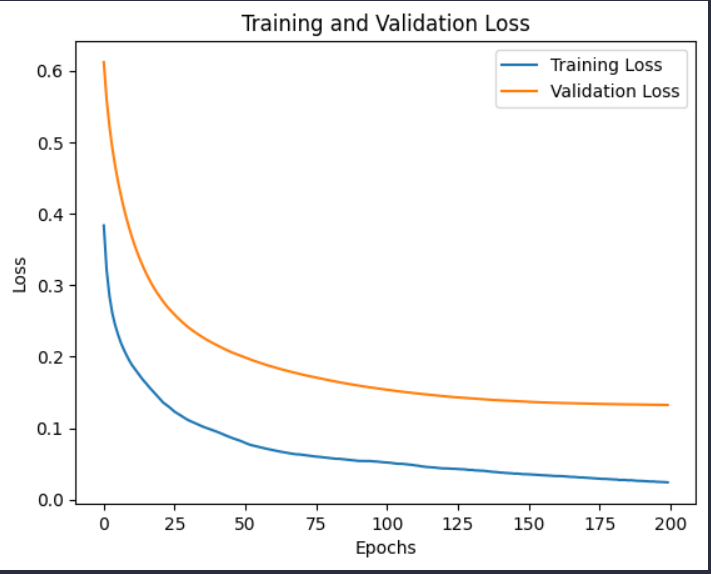
\includegraphics[width=0.75\textwidth]{Graph.PNG}
    \caption{Training and validation loss}
    \label{fig:my_pic}
\end{figure}


\subsection{(10 Puan)} \textbf{SEED=öğrenci numaranız set ettikten sonra altıncı haftada ödev olarak verdiğim gibi earlystopping'deki en iyi modeli kullanarak, Prensesi İyileştir test setinden accuracy, F1, precision ve recall değerlerini hesaplayan kodu yazın ve sonucu da aşağı yapıştırın. \%80'den fazla başarı bekliyorum test setinden. Daha düşükse başarı oranınız, nerede hata yaptığınızı bulmaya çalışın. \%90'dan fazla başarı almak mümkün (ben denedim).}

\begin{python}
trainData = pd.read_csv('./csv/cure_the_princess_train.csv')
validData = pd.read_csv('./csv/cure_the_princess_validation.csv')
testData =  pd.read_csv('./csv/cure_the_princess_test.csv')

trainX = trainData.drop(columns=['Cured']).values
trainY = trainData['Cured'].values
validX = validData.drop(columns=['Cured']).values
validY = validData['Cured'].values
testX = testData.drop(columns=['Cured']).values
testY = testData['Cured'].values

numInputFeatures = trainX.shape[1]

torch.manual_seed(190401070)

class MLP(nn.Module):
    def __init__(self, numInputFeatures):
        super().__init__()
        self.fc1 = nn.Linear(numInputFeatures, 100) 
        self.relu1 = nn.ReLU() 
        self.fc2 = nn.Linear(100, 50) 
        self.relu2 = nn.ReLU() 
        self.fc3 = nn.Linear(50, 1) 
        self.sigmoid = nn.Sigmoid() 
        
    def forward(self, x):
        x = self.fc1(x)
        x = self.relu1(x)
        x = self.fc2(x)
        x = self.relu2(x)
        x = self.fc3(x)
        x = self.sigmoid(x)
        return x
        
model = MLP(numInputFeatures=numInputFeatures)

criterion = nn.BCELoss()
optimizer = torch.optim.SGD(model.parameters(), lr=0.0006)

numEpochs = 250
batchSize = 16
trainLosses = []
validLosses = []
bestValidLoss = None
patience = 10
counter = 0

for epoch in range(numEpochs):
    for i in range(0, len(trainX), batchSize):
        
        batchX = torch.tensor(trainX[i:i+batchSize], dtype=torch.float32)
        batchY = torch.tensor(trainY[i:i+batchSize], dtype=torch.float32).view(-1, 1)
        
        outputs = model(batchX)
        loss = criterion(outputs, batchY)
        
        optimizer.zero_grad()
        loss.backward()
        optimizer.step()
        
    trainLosses.append(loss.item())
    print('Epoch [%d/%d], Training Loss: %.4f' % (epoch+1, numEpochs, loss.item()))
    
    validLoss = criterion(model(torch.tensor(validX, dtype=torch.float32)), torch.tensor(validY, dtype=torch.float32).view(-1, 1)).item()
    validLosses.append(validLoss)
    print('Epoch [%d/%d], Validation Loss: %.4f' % (epoch+1, numEpochs, validLoss))

    if bestValidLoss is None or  validLoss < bestValidLoss:
        bestValidLoss = validLoss
        counter = 0
    else:
        counter += 1
        if counter >= patience:
            print("Early stopping!!!", epoch)
            break

    with torch.no_grad():
        testOutputs = model(torch.tensor(testX, dtype=torch.float32))
        testPredictions = (testOutputs > 0.5).float().view(-1)

        
        accuracy = (testPredictions == torch.tensor(testY, dtype=torch.float32)).float().mean().item()
        precision = (testPredictions[testPredictions == 1] == torch.tensor(testY[testPredictions == 1], dtype=torch.float32)).float().mean().item()
        recall = (testPredictions[testY == 1] == torch.tensor(testY[testY == 1], dtype=torch.float32)).float().mean().item()
        f1 = 2 * precision * recall / (precision + recall)
        print('Accuracy: %.4f, Precision: %.4f, Recall: %.4f, F1: %.4f' % (accuracy, precision, recall, f1))

plt.plot(trainLosses, label='Training Loss')
plt.plot(validLosses, label='Validation Loss')
plt.xlabel('Epochs')
plt.ylabel('Loss')
plt.title('Training and Validation Loss')
plt.legend()
plt.show()
\end{python}

Earlystopping ile 222. epoch da durdurdu. En son epochda  çıkan değerler  aşağıdaki gibidir.

Accuracy: 0.9469, Precision: 0.9780, Recall: 0.9149, F1: 0.9454

\subsection{(5 Puan)} \textbf{Tüm kodların CPU'da çalışması ne kadar sürüyor hesaplayın. Sonra to device yöntemini kullanarak modeli ve verileri GPU'ya atıp kodu bir de böyle çalıştırın ve ne kadar sürdüğünü hesaplayın. Süreleri aşağıdaki tabloya koyun. GPU için Google Colab ya da Kaggle'ı kullanabilirsiniz, iki ortam da her hafta saatlerce GPU hakkı veriyor.}

\begin{table}[ht!]
    \centering
    \caption{CPU VE GPU da çalışma süreleri}
    \begin{tabular}{c|c}
        Ortam & Süre (saniye) \\\hline
        CPU & 16.95974326133728 \\
        GPU & 15.498067855834961\\
    \end{tabular}
    \label{tab:my_table}
\end{table}

\subsection{(3 Puan)} \textbf{Modelin eğitim setine overfit etmesi için elinizden geldiği kadar kodu gereken şekilde değiştirin, validasyon loss'unun açıkça yükselmeye başladığı, training ve validation loss'ları içeren figürü aşağı koyun ve overfit için yaptığınız değişiklikleri aşağı yazın. Overfit, tam bir çanak gibi olmalı ve yükselmeli. Ona göre parametrelerle oynayın.}

{Overfit etmesi için epok sayısını 250 den 1500'e kadar yükselttim ve aşağıdaki grafik ortaya çıktı.}

\begin{figure}[ht!]
   
    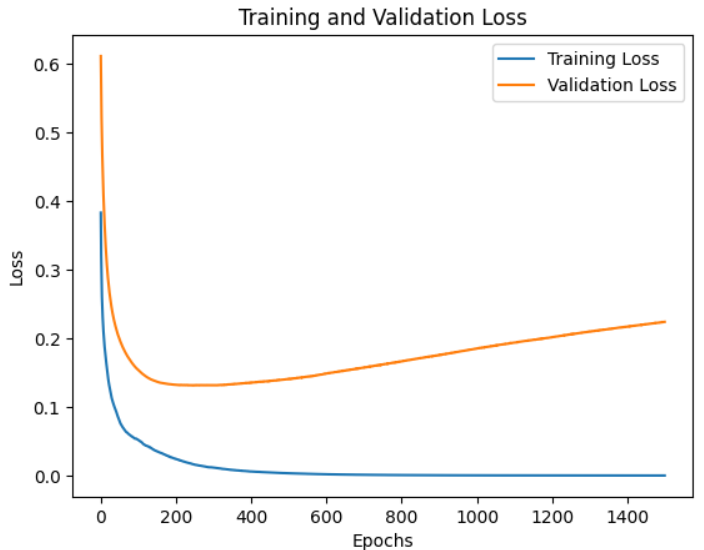
\includegraphics[width=0.75\textwidth]{overfit.PNG}
    \caption{Overfit}
    \label{fig:my_pic2}
\end{figure}





\subsection{(2 Puan)} \textbf{Beşinci soruya ait tüm kodların ve cevapların olduğu jupyter notebook'un Github linkini aşağıdaki url'e koyun.}

\url{https://github.com/EMREEGEDUKK/MultiLayerPerceptronPytorch/blob/main/mlp.ipynb}


\section{(Toplam 10 Puan)} \textbf{Bir önceki sorudaki Prensesi İyileştir problemindeki yapay sinir ağınıza seçtiğiniz herhangi iki farklı regülarizasyon yöntemi ekleyin ve aşağıdaki soruları cevaplayın.} 

\subsection{(2 puan)} \textbf{Kodlarda regülarizasyon eklediğiniz kısımları aşağı koyun:} 

\begin{python}
class MLP(nn.Module):
    def __init__(self, numInputFeatures):
        super().__init__()
        self.fc1 = nn.Linear(numInputFeatures, 100) 
        nn.init.xavier_uniform_(self.fc1.weight, gain=math.sqrt(2))
        self.relu1 = nn.ReLU() 
        self.dropout1 = nn.Dropout(p=0.1) 
        self.fc2 = nn.Linear(100, 50)
        nn.init.xavier_uniform_(self.fc2.weight, gain=math.sqrt(2))
        self.relu2 = nn.ReLU() 
        self.dropout2 = nn.Dropout(p=0.1) 
        self.fc3 = nn.Linear(50, 1) 
        nn.init.xavier_uniform_(self.fc3.weight, gain=math.sqrt(2))
        self.sigmoid = nn.Sigmoid() 
        
    def forward(self, x):
        x = self.fc1(x)
        x = self.relu1(x)
        x = self.dropout1(x)
        x = self.fc2(x)
        x = self.relu2(x)
        x = self.dropout2(x)
        x = self.fc3(x)
        x = self.sigmoid(x)
        return x
\end{python}

\subsection{(2 puan)} \textbf{Test setinden yeni accuracy, F1, precision ve recall değerlerini hesaplayıp aşağı koyun:}

Accuracy: 0.9106, Precision: 0.9299, Recall: 0.8892, F1: 0.9091

\subsection{(5 puan)} \textbf{Regülarizasyon yöntemi seçimlerinizin sebeplerini ve sonuçlara etkisini yorumlayın:}

Dropout yöntemini aşırı öğrenme problemini azaltması için kullanmak istedim. Xavier initializationı ise daha iyi öğrenmesi için ağırlık değerlerini random olarak atamak yerine bir başlangıç değerine sahip olacak şekilde atadım. Sonuçlarda ise herhangi bir artış olmadı çok küçük seviyede bir düşüş yaşandı.

\subsection{(1 puan)} \textbf{Sonucun github linkini  aşağıya koyun:}

{sonuçlar sondaki cellde bulunmaktadır. }

\url{https://github.com/EMREEGEDUKK/MultiLayerPerceptronPytorch/blob/main/mlp.ipynb}

\end{document}